The edge region is in parts a very good vacuum, so 
that the plasma ion species typically do not thermalise fully.
Nonetheless it may be adequate for many purposes to treat the majority ionised species as fluids,
although this is harder to argue for impurity species that may be present only in relatively
small numbers.
In fact, collision timescales typically vary $\tau\propto T^{3/2}/N$ where $T$ is the temperature of the species
and~$N$ is its number density, so that a species may be treatable as a fluid over say microsecond
timescales in cooler, denser regions, but not on shorter timescales or in parts closer to the core.
There is the additional complication of sheath formation at the edge, where the preferential
loss of electrons leads to strong electric fields and consequently flows close to sonic,
so that most workers model the sheath plasma using particles, typically with the Particle-in-Cell~(PIC)
approach, although for the Vlasov equation a wide range of numerical techniques has been examined,
see eg.\ Palmroth~et~al~\cite[\S\,4]{Pa18Vlas}.
\emph{N.B. Discussion in this note implies usage of particles to model kinetic effects,
not schemes such as SPH designed to model advection of classical fluids.}

The cooler parts of the tokamak edge plasma may contain large numbers of
neutral atoms.
Neutrals are generically less likely than charged species to thermalise.
They circulate into hotter and denser regions and collide with charged species.
Classical transport coefficients~$\kappa$, in
addition to a~$1/\tau$ dependence, are anisotropic because of the strong magnetic field,
to the extent that collisions with neutrals may become an important limiting mechanism
for transport along the field. Operationally the most important aspect of the
neutral species is however that because of the collisions, they
represent a source of plasma.

The non-Maxwellian or kinetic aspects of the edge may lead to a need to solve the
Boltzmann equation, in fact not only with quadratic source terms representing interaction
between two species colliding, but with cubic terms representing chemical reactions.
Classical fluid dynamics of course assumes Maxwellian dependence on phase velocity and
concentrates on the first few moments  density, mean flow and sometimes temperature
as well as pressure. It can be helpful to introduce
the concept of phase-fluid, where extra dimensions represent the velocity-space
dependence at a position in full detail.
In the phase-fluid approach, the concept of multiplicatively perturbing
a Maxwellian has been explored. The main and important advantage of this approach
is that it often facilitates massive simplification of the collision integrals
in Boltzmann, to a single point term in significant cases, eg.\ ref~\cite{zhdanov}.

Kormann, with Yurova and others (private communication, 2019) have recently reviewed the use of 
the Hermite basis (ie.\ a Gaussian multiplied by a Hermite polynomial). Two
significant works are Vencels et al.~\cite{Ve16Spec} describing Spectralplasmasolver
and J.T.Parker's thesis~\cite{jtparker} which describes software focused on
gyroaveraged kinetics, namely SPECTROGK. Note that all these works use a Fourier
representation for real space, the so-called Fourier-Hermite method.
%, so that additional development would be needed for \nep

Even with the simplification of a multiply-periodic domain,
there are nonetheless issues particularly at high velocity values
and of course a Maxwellian may not be a particularly good approximation. 
Hence, borrowing from classical CFD practice on a infinite domain, it might be
interesting to look at mappings which expand a set of compact spectral elements to cover
the whole of velocity space.

\begin{figure}
\centerline{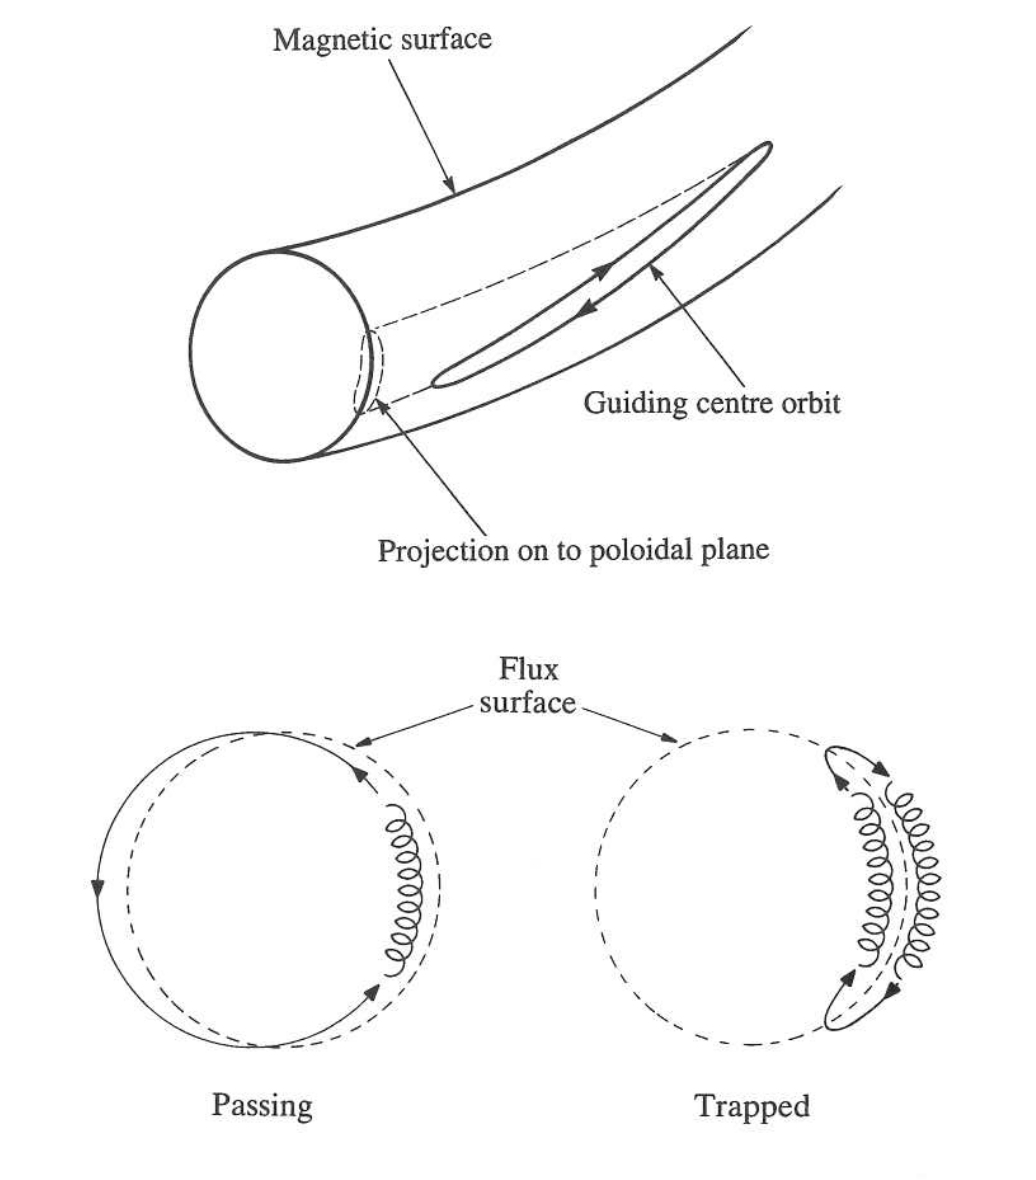
\includegraphics[width=8cm]{../png/pcle_orbits}}
\caption{Important classes of particle trajectories from Wesson~\cite[\S\,3.10]{wesson}.\label{fig:orbits}}
\end{figure}

Alternatively it may be easier to return to basics and look at a particle representation
for the ionised species as well as for the neutrals. This
may be as efficient as using higher order elements since the distribution function in velocity may not be
very smooth. As the sketch in \Fig{orbits} indicates, there are two important classes of particle
trajectories, depending on the particle energy and where in the magnetic field they begin.
The first set approximately follow the fieldlines, gyrating as they go, whereas the second set
may have trajectories that bounce. There is lack of smoothness at the trapped-passing
boundary in velocity space.


%The need to use particle as well as fluid models, puts a significant burden on the software,
%because it gives rise to a general need to be able to move between representations without
%introducing excessive error.
